% Options for packages loaded elsewhere
\PassOptionsToPackage{unicode}{hyperref}
\PassOptionsToPackage{hyphens}{url}
%
\documentclass[
]{article}
\usepackage{amsmath,amssymb}
\usepackage{lmodern}
\usepackage{iftex}
\ifPDFTeX
  \usepackage[T1]{fontenc}
  \usepackage[utf8]{inputenc}
  \usepackage{textcomp} % provide euro and other symbols
\else % if luatex or xetex
  \usepackage{unicode-math}
  \defaultfontfeatures{Scale=MatchLowercase}
  \defaultfontfeatures[\rmfamily]{Ligatures=TeX,Scale=1}
\fi
% Use upquote if available, for straight quotes in verbatim environments
\IfFileExists{upquote.sty}{\usepackage{upquote}}{}
\IfFileExists{microtype.sty}{% use microtype if available
  \usepackage[]{microtype}
  \UseMicrotypeSet[protrusion]{basicmath} % disable protrusion for tt fonts
}{}
\makeatletter
\@ifundefined{KOMAClassName}{% if non-KOMA class
  \IfFileExists{parskip.sty}{%
    \usepackage{parskip}
  }{% else
    \setlength{\parindent}{0pt}
    \setlength{\parskip}{6pt plus 2pt minus 1pt}}
}{% if KOMA class
  \KOMAoptions{parskip=half}}
\makeatother
\usepackage{xcolor}
\usepackage[margin=1.0in]{geometry}
\usepackage{graphicx}
\makeatletter
\def\maxwidth{\ifdim\Gin@nat@width>\linewidth\linewidth\else\Gin@nat@width\fi}
\def\maxheight{\ifdim\Gin@nat@height>\textheight\textheight\else\Gin@nat@height\fi}
\makeatother
% Scale images if necessary, so that they will not overflow the page
% margins by default, and it is still possible to overwrite the defaults
% using explicit options in \includegraphics[width, height, ...]{}
\setkeys{Gin}{width=\maxwidth,height=\maxheight,keepaspectratio}
% Set default figure placement to htbp
\makeatletter
\def\fps@figure{htbp}
\makeatother
\setlength{\emergencystretch}{3em} % prevent overfull lines
\providecommand{\tightlist}{%
  \setlength{\itemsep}{0pt}\setlength{\parskip}{0pt}}
\setcounter{secnumdepth}{-\maxdimen} % remove section numbering
\newlength{\cslhangindent}
\setlength{\cslhangindent}{1.5em}
\newlength{\csllabelwidth}
\setlength{\csllabelwidth}{3em}
\newlength{\cslentryspacingunit} % times entry-spacing
\setlength{\cslentryspacingunit}{\parskip}
\newenvironment{CSLReferences}[2] % #1 hanging-ident, #2 entry spacing
 {% don't indent paragraphs
  \setlength{\parindent}{0pt}
  % turn on hanging indent if param 1 is 1
  \ifodd #1
  \let\oldpar\par
  \def\par{\hangindent=\cslhangindent\oldpar}
  \fi
  % set entry spacing
  \setlength{\parskip}{#2\cslentryspacingunit}
 }%
 {}
\usepackage{calc}
\newcommand{\CSLBlock}[1]{#1\hfill\break}
\newcommand{\CSLLeftMargin}[1]{\parbox[t]{\csllabelwidth}{#1}}
\newcommand{\CSLRightInline}[1]{\parbox[t]{\linewidth - \csllabelwidth}{#1}\break}
\newcommand{\CSLIndent}[1]{\hspace{\cslhangindent}#1}
\usepackage{helvet}
\renewcommand*\familydefault{\sfdefault}
\usepackage{setspace}
\doublespacing
\usepackage[left]{lineno}
\usepackage{multirow}
\usepackage[none]{hyphenat}
\ifLuaTeX
  \usepackage{selnolig}  % disable illegal ligatures
\fi
\IfFileExists{bookmark.sty}{\usepackage{bookmark}}{\usepackage{hyperref}}
\IfFileExists{xurl.sty}{\usepackage{xurl}}{} % add URL line breaks if available
\urlstyle{same} % disable monospaced font for URLs
\hypersetup{
  pdftitle={Machine learning classification using self-reference-based OTU clustering},
  hidelinks,
  pdfcreator={LaTeX via pandoc}}

\title{\textbf{Machine learning classification using
self-reference-based OTU clustering}}
\author{}
\date{\vspace{-2.5em}}

\begin{document}
\maketitle

Running title: Reference-based OTU clustering for ML classification

\vspace{10mm}

Courtney R. Armour\({^1}\), Kelly L. Sovacool\({^2}\), William L.
Close\(^{1,*}\), Begüm D. Topçuoğlu\(^{1,\#}\), Jenna Wiens\({^3}\),
Patrick D. Schloss \(^{1,\dagger}\)

\vspace{10mm}

\({^1}\) Department of Microbiology and Immunology, University of
Michigan, Ann Arbor, Michigan, USA

\({^2}\) Department of Computational Medicine and Bioinformatics,
University of Michigan, Ann Arbor, Michigan, USA

\({^3}\) Department of Electrical Engineering and Computer Science,
University of Michigan, Ann Arbor, Michigan, USA

\({^*}\) Current Affiliation: Bio-Rad Laboratories, Hercules,
California, USA

\({^\#}\) Current Affiliation: Bristol Myers Squibb, Summit, New Jersey,
USA

\(\dagger\) To whom correspondence should be addressed:
\href{mailto:pschloss@umich.edu}{\nolinkurl{pschloss@umich.edu}}

\vspace{10mm}

\textbf{observation format} (max 1200 words, 2 figures, 25 ref)

\newpage

\linenumbers

\hypertarget{abstract}{%
\subsection{Abstract}\label{abstract}}

Machine learning classification using the gut microbiome relies on
assigning 16S rRNA gene sequences into operational taxonomic units
(OTUs) to quantify microbial composition. OTU abundances are then used
to train a classification model that can be applied to classify new
samples. The standard approaches to clustering sequences include
reference-based and \emph{de novo} clustering. Reference-based
clustering requires a well-curated reference database that may not exist
for all systems. \emph{De novo} clustering tends to produce higher
quality OTU assignments than reference-based, but clusters depend on the
sequences in the dataset and therefore OTU assignments will change when
new samples are sequenced. This lack of stability complicates machine
learning classification since new sequences must be reclustered with the
old data and the model retrained with the new OTU assignments. The
OptiFit algorithm addresses these issues by fitting new sequences into
existing OTUs. While OptiFit produces high quality OTU clusters, it is
unclear whether this method for fitting new sequence data into existing
OTUs will impact the performance of classification models trained with
the older data. We used OptiFit to cluster sequences into existing OTUs
and evaluated model performance in classifying a dataset containing
samples from patients with and without colonic screen relevant neoplasia
(SRN). We compared the performance of this model to standard methods
including \emph{de novo} and database-reference-based clustering. We
found that using OptiFit performed as well or better in classifying
SRNs. OptiFit can streamline the process of classifying new samples by
avoiding the need to retrain models using reclustered sequences.

\hypertarget{importance}{%
\subsection{Importance}\label{importance}}

There is great potential for using microbiome data to aid in diagnosis.
A challenge with OTU-based classification models is that 16S rRNA gene
sequences are often assigned to OTUs based on similarity to other
sequences in the dataset. If data are generated from new patients, the
old and new sequences must all be reassigned to OTUs and the
classification model retrained. Yet there is a desire to have a single,
validated model that can be widely deployed. To overcome this obstacle,
we applied the OptiFit clustering algorithm to fit new sequence data to
existing OTUs allowing for reuse of the model. A random forest model
implemented using OptiFit performed as well as the traditional reassign
and retrain approach. This result shows that it is possible to train and
apply machine learning models based on OTU relative abundance data that
do not require retraining or the use of a reference database.

\newpage

There is increasing evidence for an association between the composition
of the gut microbiome and a variety of diseases, such as crohn's disease
and colorectal cancer. The signatures that associate with disease have
shown potential to aid in diagnosis of disease throught gut microbiome
profiling and machine learning. Taxonomic composition of microbial
communities can be assessed using amplicon sequencing of the 16S rRNA
gene, which is the input to classification models. Analysis of 16S rRNA
gene sequence data generally relies on assigning sequences into
operational taxonomic units (OTUs). The process of OTU clustering can
either be reference-based or \emph{de novo}. The quality of OTUs
generated with reference-based clustering is generally poor compared to
those generated with \emph{de novo} clustering
(\protect\hyperlink{ref-westcott2015}{1}). While \emph{de novo}
clustering produces high-quality OTU clusters where sequences are
accurately grouped based on similarity thresholds, the resulting OTU
clusters depend on the sequences within the dataset and the addition of
new data has the potential to redefine OTU cluster composition. The
unstable nature of \emph{de novo} OTU clustering complicates deployment
of machine learning models since integration of additional data requires
reclustering all the data and retraining the model. The ability to
integrate new data into a validated model without reclustering and
retraining could allow for the application of a single model that can
continually classify new data. Recently, Sovacool \emph{et al.}
introduced OptiFit, a method for fitting new sequence data into existing
OTUs (\protect\hyperlink{ref-sovacool2022}{2}). While OptiFit can
effectively fit new sequence data to existing OTU clusters, it is
unknown if the use of OptiFit will have an impact on classification
performance. Here, we tested the ability of OptiFit to cluster new
sequence data into existing OTU clusters for the purpose of classifying
disease based on gut microbiome composition.

We compared the ability of several approaches for assigning 16S rRNA
gene seequences to OTUs including, \emph{de novo},
database-reference-based, and self-reference-based with OptiFit. To test
how the model performance compared between these approaches, we used a
publicly available dataset of 16S rRNA gene sequences from stool samples
of healthy subjects (n = 226) as well as subjects with screen-relevant
neoplasia (SRN) consisting of advanced adenoma and carcinoma (n = 229)
(\protect\hyperlink{ref-baxter2016}{3}). For the \emph{de novo}
workflows, all the 16S rRNA sequence data was clustered into OTUs. The
OTU clustering was conducted using two common algorithms: 1) the
OptiClust algorithm in mothur 1 and 2) the VSEARCH algorithm used in
QIIME2 (\protect\hyperlink{ref-rognes2016}{4},
\protect\hyperlink{ref-bolyen2019}{5}). For both algorithms, the
resulting abundance data was then split into training and testing sets,
where the training set was used to tune hyperparameters and ultimately
train and select the model. The model was applied to the testing set and
performance evaluated (Figure 1A). We also conducted reference-based OTU
clustering using OptiFit to fit the sequence data into OTUs based on the
greengenes reference database. To compare with another commonly used
method, we also used the VSEARCH algorithm to fit the sequence data to
the greengenes reference (Figure 1B). In the OptiFit self-reference
workflow, the data was split into a training and a testing set. The
training set was clustered into OTUs and used to train a classification
model. The OptiFit algorithm was used to fit sequence data of samples
not part of the original dataset into the existing OTUs, and used the
same model to classify the samples (Figure 1C). For each of the
workflows the process was repeated for 100 random splits of the data to
account for variation caused by the choice of the random number
generator seed.

We first examined the quality of the resulting OTU clusters from each
method using the Matthews correlation coefficient (MCC). MCC is a metric
used to measure OTU cluster quality based on the similarity of all pairs
of sequences and whether they are appropriately clustered or not
(\protect\hyperlink{ref-westcott2015}{1}). MCC scores range between
negative one and one, and measure how well clustering assignment
correlates with the distance between sequences. To ensure that OptiFit
appropriately integrated new sequence data into the existing OTUs, we
expected the MCC scores produced by the OptiFit workflow to be similar
to that of \emph{de novo} clustering using the OptiClust algorithm. In
the OptiFit workflow the test data was fit to the clustered training
data for each of the 100 data splits resulting in an MCC score for each
split of the data. In the remaining workflows, the data was only
clustered once and then split into the training and testing sets
resulting in a single MCC score for each method. Indeed, the MCC scores
were similar between the OptiClust \emph{de novo} (MCC = 0.884) and
OptiFit self-reference workflows (average MCC = 0.879, standard
deviation = 0.002). Previously, we observed that \emph{de novo}
clustering tends to produce higher MCC scores than reference-based
clustering (\protect\hyperlink{ref-sovacool2022}{2}). Consistent with
prior findings the reference-based methods produced lower MCC scores
(OptiFit Greengenes MCC = 0.786; VSEARCH Greengenes MCC = 0.531) than
the \emph{de novo} methods with the same algorithm (OptiClust \emph{de
novo} MCC = 0.884; VSEARCH \emph{de novo} MCC = 0.641). Another metric
we examined for the OptiFit workflow was the fraction of sequences from
the test set that mapped to the reference OTUs. Since sequences that did
not map to reference OTUs were eliminated, if a high percentage of reads
did not map to an OTU we expected this loss of data to negatively impact
classification performance. We found that loss of data was not an issue
since on average 99.8\% (standard deviation = 0.68\%) of sequences in
the test set mapped to the reference OTUs. This number is higher than
the average fraction of reads mapped in the OptiFit Greengenes workflow
( 96.8\% +/- 3.5). These results indicate that the OptiFit
self-reference method performed as well as the OptiClust \emph{de novo}
method and better than using an external database.

We next assessed model performance using OTU relative abundances from
the training data from the workflows to train a model to predict SRNs
and used the model on the held out data. Using the predicted and actual
diagnosis classification, we calculated the area under the receiver
operating characteristic curve (AUROC) for each data split. During
cross-validation (CV) training, the model performance was equivalent
between OptFit self-reference and OptiClust \emph{de novo} (p-value =
0.071; Figure 2A) while while performance for both VSEARCH methods was
lower than the OptiClust \emph{de novo}, OptiFit self, and OptiFit
Greengenes methods (p-values \textless{} 0.05). The trained model was
then applied to the test data classifying samples as either control or
SRN. Both VSEARCH methods perform slightly worse than the OptiClust *de
novo* method (both p-values \textless{} 0.05). However the performance
on the test data was equivalent between the OptiClust \emph{de novo},
OptiFit Greengenes, and OptiFit self-reference approaches (p-value
\textgreater{} 0.05; Figures 2B and 2C). These results indicate that new
data could be fit to existing OTU clusters using OptiFit without
impacting model performance.

We tested the ability of OptiFit to integrate new data into existing
OTUs for the purpose of machine learning classification using OTU
relative abundance. A potential problem with using OptiFit is that any
sequences from the new samples that do not map to the existing OTU
clusters will be discarded, resulting in a possible loss of information.
However, we demonstrated that OptiFit can be used to fit new sequence
data into existing OTU clusters and it could perform as well in
predicting SRN compared to \emph{de novo} clustering all the sequence
data together. In this instance, the performance of OptiFit was
equivalent to using a database-reference-based method despite the lower
quality of the OTU clusters in the database-reference-based approach.
This likely indicates that the sequences that are important to the model
are well characterized by the reference database. However, a less well
studied system may not be as well characterized by a reference-database
which would make the ability to utilize one's own data a reference an
exciting possiblility. The ability to integrate data from new samples
into existing OTUs enables the implementation of a single machine
learning model. This is important for model implementation because not
all of the data needs to be available or known at the time of model
generation. A robust machine learning model can be implemented as part
of a non-invasive and low-cost diagnostic for SRN and other diseases.

\hypertarget{materials-and-methods}{%
\subsection{Materials and Methods}\label{materials-and-methods}}

\textbf{Dataset.} Raw 16S rRNA gene sequence data from the V4 region
were previously generated from human stool samples. Sequences were
downloaded from the NCBI Sequence Read Archive (accession no. SRP062005)
(\protect\hyperlink{ref-baxter2016}{3},
\protect\hyperlink{ref-edgar2011}{6}). This dataset contains stool
samples from 490 subjects. For this analysis, samples from subjects
identified in the metadata as normal, high risk normal, or adenoma were
categorized as ``normal'', while samples from subjects identified as
advanced adenoma or carcinoma were categorized as ``screen relevant
neoplasia'' (SRN). The resulting dataset consisted of 261 normal samples
and 229 SRN samples.

\textbf{Data processing.} The full dataset was preprocessed with mothur
(v1.47) (\protect\hyperlink{ref-schloss2009}{7}) to join forward and
reverse reads, merge duplicate reads, align to the SILVA reference
database (v132) (\protect\hyperlink{ref-quast2013}{8}), precluster,
remove chimeras with UCHIME (\protect\hyperlink{ref-edgar2011}{6}),
assign taxonomy, and remove non-bacterial reads following the Schloss
Lab MiSeq standard operating procedure described on the mothur website
(\url{https://mothur.org/wiki/miseq_sop/}). 100 splits of the 490
samples were generated where 80\% of the samples (392 samples) were
randomly assigned to the training set and the remaining 20\% (98
samples) were assigned to the test set. Using 100 splits of the data
accounts for the variation that may be observed depending on the samples
that are in the training or test sets. Each sample was in the training
set an average of 80 times (standard deviation = 4.1) and the test set
an average of 20 times (standard deviation = 4.1`).

\textbf{\emph{Reference-based workflows.}}

\begin{enumerate}
\def\labelenumi{\arabic{enumi}.}
\tightlist
\item
  OptiFit Self: The preprocess data was split into the training and
  testing sets. The training set was clustered into OTUs using
  OptiClust, then the test set was fit to the OTUs of the training set
  using the OptiFit algorithm (\protect\hyperlink{ref-sovacool2022}{2}).
  The OptiFit algorithm was run with method open so that any sequences
  that did not map to the existing OTU clusters would form new OTUs. The
  data was then subsampled to 10,000 reads and any novel OTUs from the
  test set were removed. This process was repeated for each of the 100
  splits resulting in 100 training and testing datasets.
\item
  OptiFit Greengenes: Reference sequences from the Greengenes database
  v13\_8\_99 (\protect\hyperlink{ref-desantis2006}{9}) were downloaded
  and processed with mothur by trimming to the V4 region and clustered
  \emph{de novo} with OptiClust

  \begin{enumerate}
  \def\labelenumii{\arabic{enumii}.}
  \tightlist
  \item
    The preprocessed data was fit to the clustered reference data using
    OptiFit with the method open to allow any sequences that did not map
    to the existing reference clusters would form new OTUs. The data was
    then subsampled to 10,000 reads and any novel OTUs from the test set
    were removed. The data set was then split into two sets where 80\%
    of the samples were assigned to the training set and 20\% to the
    testing set. This process was repeated for each of the 100 splits
    resulting in 100 training and testing datasets.
  \end{enumerate}
\item
  VSEARCH Greengenes: Preprocessed data was clustered using VSEARCH
  v2.15.2 (\protect\hyperlink{ref-rognes2016}{4}) directly to
  unprocessed Greengenes 97\% OTU reference alignment consistent with
  how VSEARCH is typically used by the QIIME2 software for
  reference-based clustering (\protect\hyperlink{ref-bolyen2019}{5}).
  The data was then subsampled to 10,000 reads and any novel OTUs from
  the test set were removed. The data set was then split into two sets
  where 80\% of the samples were assigned to the training set and 20\%
  to the testing set. This process was repeated for each of the 100
  splits resulting in 100 training and testing datasets.
\end{enumerate}

\textbf{\emph{De novo workflows.}}

\begin{enumerate}
\def\labelenumi{\arabic{enumi}.}
\setcounter{enumi}{3}
\item
  OptiClust \emph{de novo}: All the preprocessed data was clustered
  together with OptiClust 1 to generate OTUs. The data was subsampled to
  10,000 reads per sample and the resulting abundance tables were split
  into the training and testing sets. The process was repeated for each
  of the 100 splits resulting in 100 training and testing datasets.
\item
  VSEARCH \emph{de novo}: All the preprocessed data was clustered using
  VSEARCH v2.15.2 (\protect\hyperlink{ref-rognes2016}{4}) with 97\%
  identity and then subsampled to 10,000 reads per sample. The process
  was repeated for each of the 100 splits resulting in 100 training and
  testing datasets for both workflows.
\end{enumerate}

\textbf{\emph{Machine Learning.}} A random forest model was trained with
the R package mikrompl (v 1.2.0)
(\protect\hyperlink{ref-topuxe7uoglu2021}{10}) to predict the diagnosis
(SRN or normal) for the samples in the test set for each data split. The
training set was preprocessed to normalize OTU counts (scale and
center), collapse correlated OTUs, and remove OTUs with zero variance.
The preprocessing from the training set was then applied to the test
set. Any OTUs in the test set that were not in the training set were
removed. P values comparing model performance were calculated as
previously described (\protect\hyperlink{ref-topuxe7uoglu2020}{11}). The
averaged ROC curves were plotted by taking the average and standard
deviation of the sensitivity at each specificity value.

\textbf{\emph{Code Availability.}}

The analysis workflow was implemented in Snakemake
(\protect\hyperlink{ref-koster2012}{12}). Scripts for analysis were
written in R (\protect\hyperlink{ref-R2020}{13}) and GNU bash
(\protect\hyperlink{ref-GNUbash}{14}). The software used includes mothur
v1.47.0 (\protect\hyperlink{ref-schloss2009}{7}), VSEARCH v2.15.2
(\protect\hyperlink{ref-rognes2016}{4}), RStudio
(\protect\hyperlink{ref-RStudio2019}{15}), the Tidyverse metapackage
(\protect\hyperlink{ref-wickham2019}{16}), R Markdown
(\protect\hyperlink{ref-xie_r_2018}{17}), the SRA toolkit
(\protect\hyperlink{ref-noauthor_sra-tools_nodate}{18}), and conda
(\protect\hyperlink{ref-noauthor_anaconda_2016}{19}). The complete
workflow and supporting files required to reproduce this study are
available at:
\url{https://github.com/SchlossLab/Armour_OptiFitGLNE_mBio_2023}

\hypertarget{acknowledgments}{%
\subsection{Acknowledgments}\label{acknowledgments}}

This work was supported through a grant from the NIH (R01CA215574).

\newpage

\hypertarget{references}{%
\subsection{References}\label{references}}

\setlength{\parindent}{-0.25in}
\setlength{\leftskip}{0.25in}

\noindent

\hypertarget{refs}{}
\begin{CSLReferences}{0}{1}
\leavevmode\vadjust pre{\hypertarget{ref-westcott2015}{}}%
\CSLLeftMargin{1. }%
\CSLRightInline{\textbf{Westcott SL}, \textbf{Schloss PD}. 2015. De novo
clustering methods outperform reference-based methods for assigning 16S
rRNA gene sequences to operational taxonomic units. PeerJ
\textbf{3}:e1487.
doi:\href{https://doi.org/10.7717/peerj.1487}{10.7717/peerj.1487}.}

\leavevmode\vadjust pre{\hypertarget{ref-sovacool2022}{}}%
\CSLLeftMargin{2. }%
\CSLRightInline{\textbf{Sovacool KL}, \textbf{Westcott SL},
\textbf{Mumphrey MB}, \textbf{Dotson GA}, \textbf{Schloss PD}. 2022.
OptiFit: An improved method for fitting amplicon sequences to existing
OTUs. mSphere \textbf{7}:e00916--21.
doi:\href{https://doi.org/10.1128/msphere.00916-21}{10.1128/msphere.00916-21}.}

\leavevmode\vadjust pre{\hypertarget{ref-baxter2016}{}}%
\CSLLeftMargin{3. }%
\CSLRightInline{\textbf{Baxter NT}, \textbf{Ruffin MT}, \textbf{Rogers
MAM}, \textbf{Schloss PD}. 2016. Microbiota-based model improves the
sensitivity of fecal immunochemical test for detecting colonic lesions.
Genome Medicine \textbf{8}:37.
doi:\href{https://doi.org/10.1186/s13073-016-0290-3}{10.1186/s13073-016-0290-3}.}

\leavevmode\vadjust pre{\hypertarget{ref-rognes2016}{}}%
\CSLLeftMargin{4. }%
\CSLRightInline{\textbf{Rognes T}, \textbf{Flouri T}, \textbf{Nichols
B}, \textbf{Quince C}, \textbf{Mahé F}. 2016. VSEARCH: a versatile open
source tool for metagenomics. PeerJ \textbf{4}:e2584.
doi:\href{https://doi.org/10.7717/peerj.2584}{10.7717/peerj.2584}.}

\leavevmode\vadjust pre{\hypertarget{ref-bolyen2019}{}}%
\CSLLeftMargin{5. }%
\CSLRightInline{\textbf{Bolyen E}, \textbf{Rideout JR}, \textbf{Dillon
MR}, \textbf{Bokulich NA}, \textbf{Abnet CC}, \textbf{Al-Ghalith GA},
\textbf{Alexander H}, \textbf{Alm EJ}, \textbf{Arumugam M},
\textbf{Asnicar F}, \textbf{Bai Y}, \textbf{Bisanz JE},
\textbf{Bittinger K}, \textbf{Brejnrod A}, \textbf{Brislawn CJ},
\textbf{Brown CT}, \textbf{Callahan BJ}, \textbf{Caraballo-Rodríguez
AM}, \textbf{Chase J}, \textbf{Cope EK}, \textbf{Da Silva R},
\textbf{Diener C}, \textbf{Dorrestein PC}, \textbf{Douglas GM},
\textbf{Durall DM}, \textbf{Duvallet C}, \textbf{Edwardson CF},
\textbf{Ernst M}, \textbf{Estaki M}, \textbf{Fouquier J},
\textbf{Gauglitz JM}, \textbf{Gibbons SM}, \textbf{Gibson DL},
\textbf{Gonzalez A}, \textbf{Gorlick K}, \textbf{Guo J},
\textbf{Hillmann B}, \textbf{Holmes S}, \textbf{Holste H},
\textbf{Huttenhower C}, \textbf{Huttley GA}, \textbf{Janssen S},
\textbf{Jarmusch AK}, \textbf{Jiang L}, \textbf{Kaehler BD},
\textbf{Kang KB}, \textbf{Keefe CR}, \textbf{Keim P}, \textbf{Kelley
ST}, \textbf{Knights D}, \textbf{Koester I}, \textbf{Kosciolek T},
\textbf{Kreps J}, \textbf{Langille MGI}, \textbf{Lee J}, \textbf{Ley R},
\textbf{Liu Y-X}, \textbf{Loftfield E}, \textbf{Lozupone C},
\textbf{Maher M}, \textbf{Marotz C}, \textbf{Martin BD},
\textbf{McDonald D}, \textbf{McIver LJ}, \textbf{Melnik AV},
\textbf{Metcalf JL}, \textbf{Morgan SC}, \textbf{Morton JT},
\textbf{Naimey AT}, \textbf{Navas-Molina JA}, \textbf{Nothias LF},
\textbf{Orchanian SB}, \textbf{Pearson T}, \textbf{Peoples SL},
\textbf{Petras D}, \textbf{Preuss ML}, \textbf{Pruesse E},
\textbf{Rasmussen LB}, \textbf{Rivers A}, \textbf{Robeson MS},
\textbf{Rosenthal P}, \textbf{Segata N}, \textbf{Shaffer M},
\textbf{Shiffer A}, \textbf{Sinha R}, \textbf{Song SJ}, \textbf{Spear
JR}, \textbf{Swafford AD}, \textbf{Thompson LR}, \textbf{Torres PJ},
\textbf{Trinh P}, \textbf{Tripathi A}, \textbf{Turnbaugh PJ},
\textbf{Ul-Hasan S}, \textbf{Hooft JJJ van der}, \textbf{Vargas F},
\textbf{Vázquez-Baeza Y}, \textbf{Vogtmann E}, \textbf{Hippel M von},
\textbf{Walters W}, \textbf{Wan Y}, \textbf{Wang M}, \textbf{Warren J},
\textbf{Weber KC}, \textbf{Williamson CHD}, \textbf{Willis AD},
\textbf{Xu ZZ}, \textbf{Zaneveld JR}, \textbf{Zhang Y}, \textbf{Zhu Q},
\textbf{Knight R}, \textbf{Caporaso JG}. 2019. Reproducible,
interactive, scalable and extensible microbiome data science using QIIME
2. Nature Biotechnology \textbf{37}:852--857.
doi:\href{https://doi.org/10.1038/s41587-019-0209-9}{10.1038/s41587-019-0209-9}.}

\leavevmode\vadjust pre{\hypertarget{ref-edgar2011}{}}%
\CSLLeftMargin{6. }%
\CSLRightInline{\textbf{Edgar RC}, \textbf{Haas BJ}, \textbf{Clemente
JC}, \textbf{Quince C}, \textbf{Knight R}. 2011. UCHIME improves
sensitivity and speed of chimera detection. Bioinformatics
\textbf{27}:2194--2200.
doi:\href{https://doi.org/10.1093/bioinformatics/btr381}{10.1093/bioinformatics/btr381}.}

\leavevmode\vadjust pre{\hypertarget{ref-schloss2009}{}}%
\CSLLeftMargin{7. }%
\CSLRightInline{\textbf{Schloss PD}, \textbf{Westcott SL},
\textbf{Ryabin T}, \textbf{Hall JR}, \textbf{Hartmann M},
\textbf{Hollister EB}, \textbf{Lesniewski RA}, \textbf{Oakley BB},
\textbf{Parks DH}, \textbf{Robinson CJ}, \textbf{Sahl JW}, \textbf{Stres
B}, \textbf{Thallinger GG}, \textbf{Van Horn DJ}, \textbf{Weber CF}.
2009. Introducing mothur: Open-source, platform-independent,
community-supported software for describing and comparing microbial
communities. Applied and Environmental Microbiology
\textbf{75}:7537--7541.
doi:\href{https://doi.org/10.1128/AEM.01541-09}{10.1128/AEM.01541-09}.}

\leavevmode\vadjust pre{\hypertarget{ref-quast2013}{}}%
\CSLLeftMargin{8. }%
\CSLRightInline{\textbf{Quast C}, \textbf{Pruesse E}, \textbf{Yilmaz P},
\textbf{Gerken J}, \textbf{Schweer T}, \textbf{Yarza P}, \textbf{Peplies
J}, \textbf{Glöckner FO}. 2013. The SILVA ribosomal RNA gene database
project: Improved data processing and web-based tools. Nucleic Acids
Research \textbf{41}:D590--D596.
doi:\href{https://doi.org/10.1093/nar/gks1219}{10.1093/nar/gks1219}.}

\leavevmode\vadjust pre{\hypertarget{ref-desantis2006}{}}%
\CSLLeftMargin{9. }%
\CSLRightInline{\textbf{DeSantis TZ}, \textbf{Hugenholtz P},
\textbf{Larsen N}, \textbf{Rojas M}, \textbf{Brodie EL}, \textbf{Keller
K}, \textbf{Huber T}, \textbf{Dalevi D}, \textbf{Hu P}, \textbf{Andersen
GL}. 2006. Greengenes, a chimera-checked 16S rRNA gene database and
workbench compatible with ARB. Applied and Environmental Microbiology
\textbf{72}:5069--5072.
doi:\href{https://doi.org/10.1128/AEM.03006-05}{10.1128/AEM.03006-05}.}

\leavevmode\vadjust pre{\hypertarget{ref-topuxe7uoglu2021}{}}%
\CSLLeftMargin{10. }%
\CSLRightInline{\textbf{Topçuoğlu BD}, \textbf{Lapp Z}, \textbf{Sovacool
KL}, \textbf{Snitkin E}, \textbf{Wiens J}, \textbf{Schloss PD}. 2021.
mikropml: User-Friendly R Package for Supervised Machine Learning
Pipelines. Journal of Open Source Software \textbf{6}:3073.
doi:\href{https://doi.org/10.21105/joss.03073}{10.21105/joss.03073}.}

\leavevmode\vadjust pre{\hypertarget{ref-topuxe7uoglu2020}{}}%
\CSLLeftMargin{11. }%
\CSLRightInline{\textbf{Topçuoğlu BD}, \textbf{Lesniak NA},
\textbf{Ruffin MT}, \textbf{Wiens J}, \textbf{Schloss PD}. 2020. A
framework for effective application of machine learning to
microbiome-based classification problems. mBio \textbf{11}:e00434--20.
doi:\href{https://doi.org/10.1128/mBio.00434-20}{10.1128/mBio.00434-20}.}

\leavevmode\vadjust pre{\hypertarget{ref-koster2012}{}}%
\CSLLeftMargin{12. }%
\CSLRightInline{\textbf{Koster J}, \textbf{Rahmann S}. 2012.
Snakemake--a scalable bioinformatics workflow engine. Bioinformatics
\textbf{28}:2520--2522.
doi:\href{https://doi.org/10.1093/bioinformatics/bts480}{10.1093/bioinformatics/bts480}.}

\leavevmode\vadjust pre{\hypertarget{ref-R2020}{}}%
\CSLLeftMargin{13. }%
\CSLRightInline{\textbf{R Core Team}. 2020.
\href{https://www.R-project.org/}{R: A language and environment for
statistical computing}. R Foundation for Statistical Computing, Vienna,
Austria.}

\leavevmode\vadjust pre{\hypertarget{ref-GNUbash}{}}%
\CSLLeftMargin{14. }%
\CSLRightInline{\textbf{GNU Project}.
\href{https://www.gnu.org/software/bash/\%20manual/bash.html/}{Bash
reference manual}.}

\leavevmode\vadjust pre{\hypertarget{ref-RStudio2019}{}}%
\CSLLeftMargin{15. }%
\CSLRightInline{\textbf{RStudio Team}. 2019.
\href{http://www.rstudio.com/}{RStudio: Integrated development
environment for r}. RStudio, Inc., Boston, MA.}

\leavevmode\vadjust pre{\hypertarget{ref-wickham2019}{}}%
\CSLLeftMargin{16. }%
\CSLRightInline{\textbf{Wickham H}, \textbf{Averick M}, \textbf{Bryan
J}, \textbf{Chang W}, \textbf{McGowan LD}, \textbf{François R},
\textbf{Grolemund G}, \textbf{Hayes A}, \textbf{Henry L}, \textbf{Hester
J}, \textbf{Kuhn M}, \textbf{Pedersen TL}, \textbf{Miller E},
\textbf{Bache SM}, \textbf{Müller K}, \textbf{Ooms J}, \textbf{Robinson
D}, \textbf{Seidel DP}, \textbf{Spinu V}, \textbf{Takahashi K},
\textbf{Vaughan D}, \textbf{Wilke C}, \textbf{Woo K}, \textbf{Yutani H}.
2019. Welcome to the Tidyverse. Journal of Open Source Software
\textbf{4}:1686.
doi:\href{https://doi.org/10.21105/joss.01686}{10.21105/joss.01686}.}

\leavevmode\vadjust pre{\hypertarget{ref-xie_r_2018}{}}%
\CSLLeftMargin{17. }%
\CSLRightInline{\textbf{Xie Y}, \textbf{Allaire JJ}, \textbf{Grolemund
G}. 2018. R {Markdown}: {The Definitive Guide}. {Taylor \& Francis, CRC
Press}.}

\leavevmode\vadjust pre{\hypertarget{ref-noauthor_sra-tools_nodate}{}}%
\CSLLeftMargin{18. }%
\CSLRightInline{{SRA}-{Tools} - {NCBI}.
http://ncbi.github.io/sra-tools/.}

\leavevmode\vadjust pre{\hypertarget{ref-noauthor_anaconda_2016}{}}%
\CSLLeftMargin{19. }%
\CSLRightInline{2016. Anaconda {Software Distribution}. Anaconda
Documentation. Anaconda Inc.}

\end{CSLReferences}

\setlength{\parindent}{0in}
\setlength{\leftskip}{0in}

\newpage

\hypertarget{figures}{%
\subsection{Figures}\label{figures}}

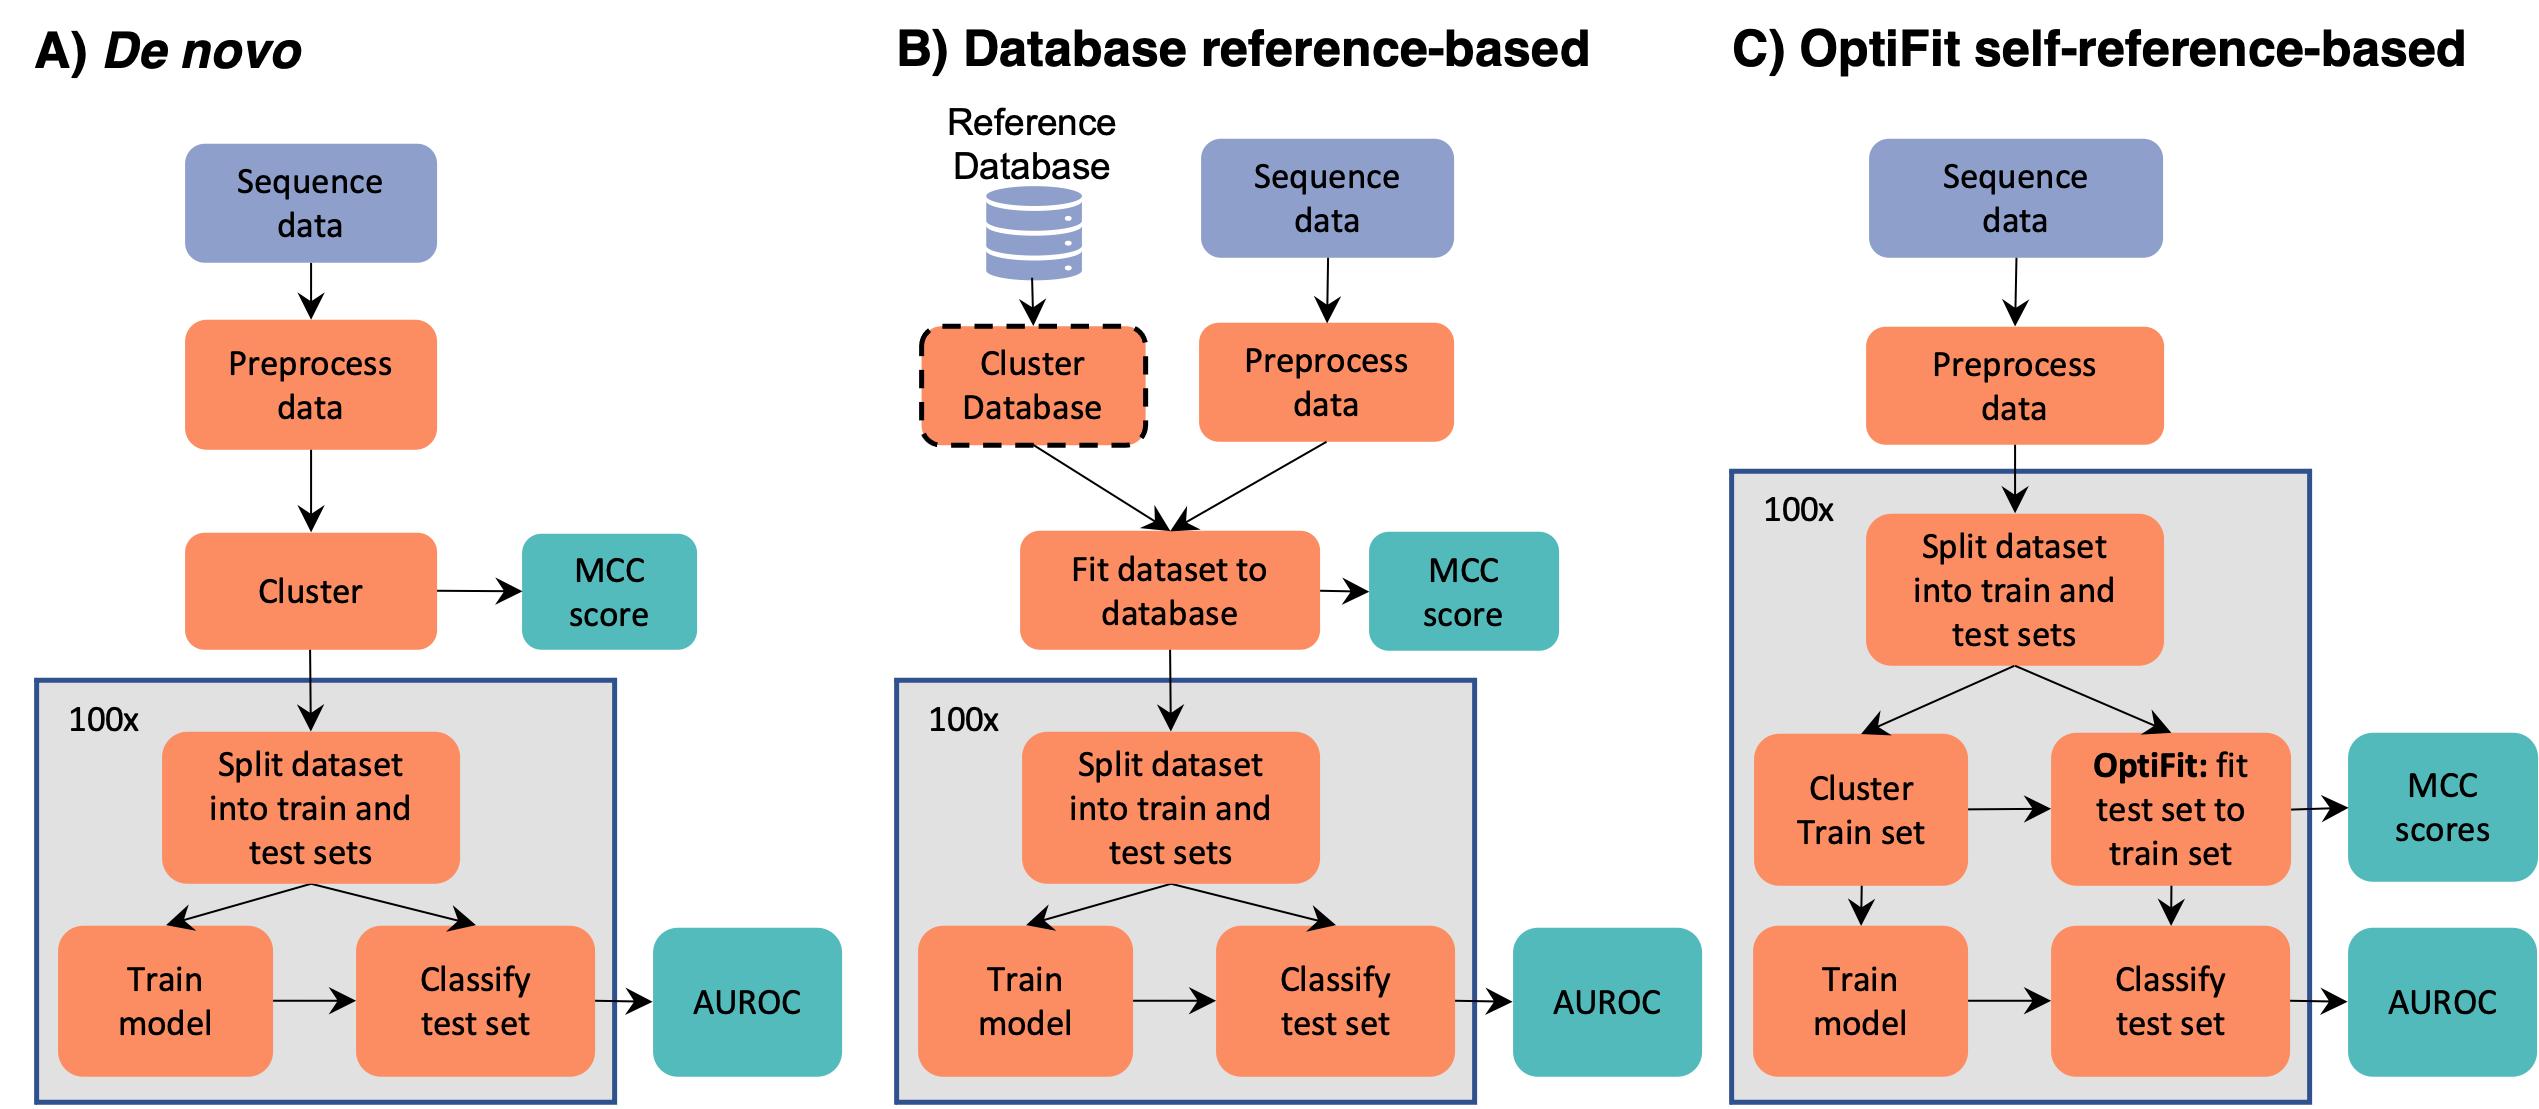
\includegraphics{./figures/Figure1.png}

\textbf{Figure1: Overview of clustering workflows.} The \emph{de novo}
and database-reference-based workflows were conducted using two
approaches: OptiClust with mothur and VSEARCH as is used in the QIIME
pipeline.

\newpage

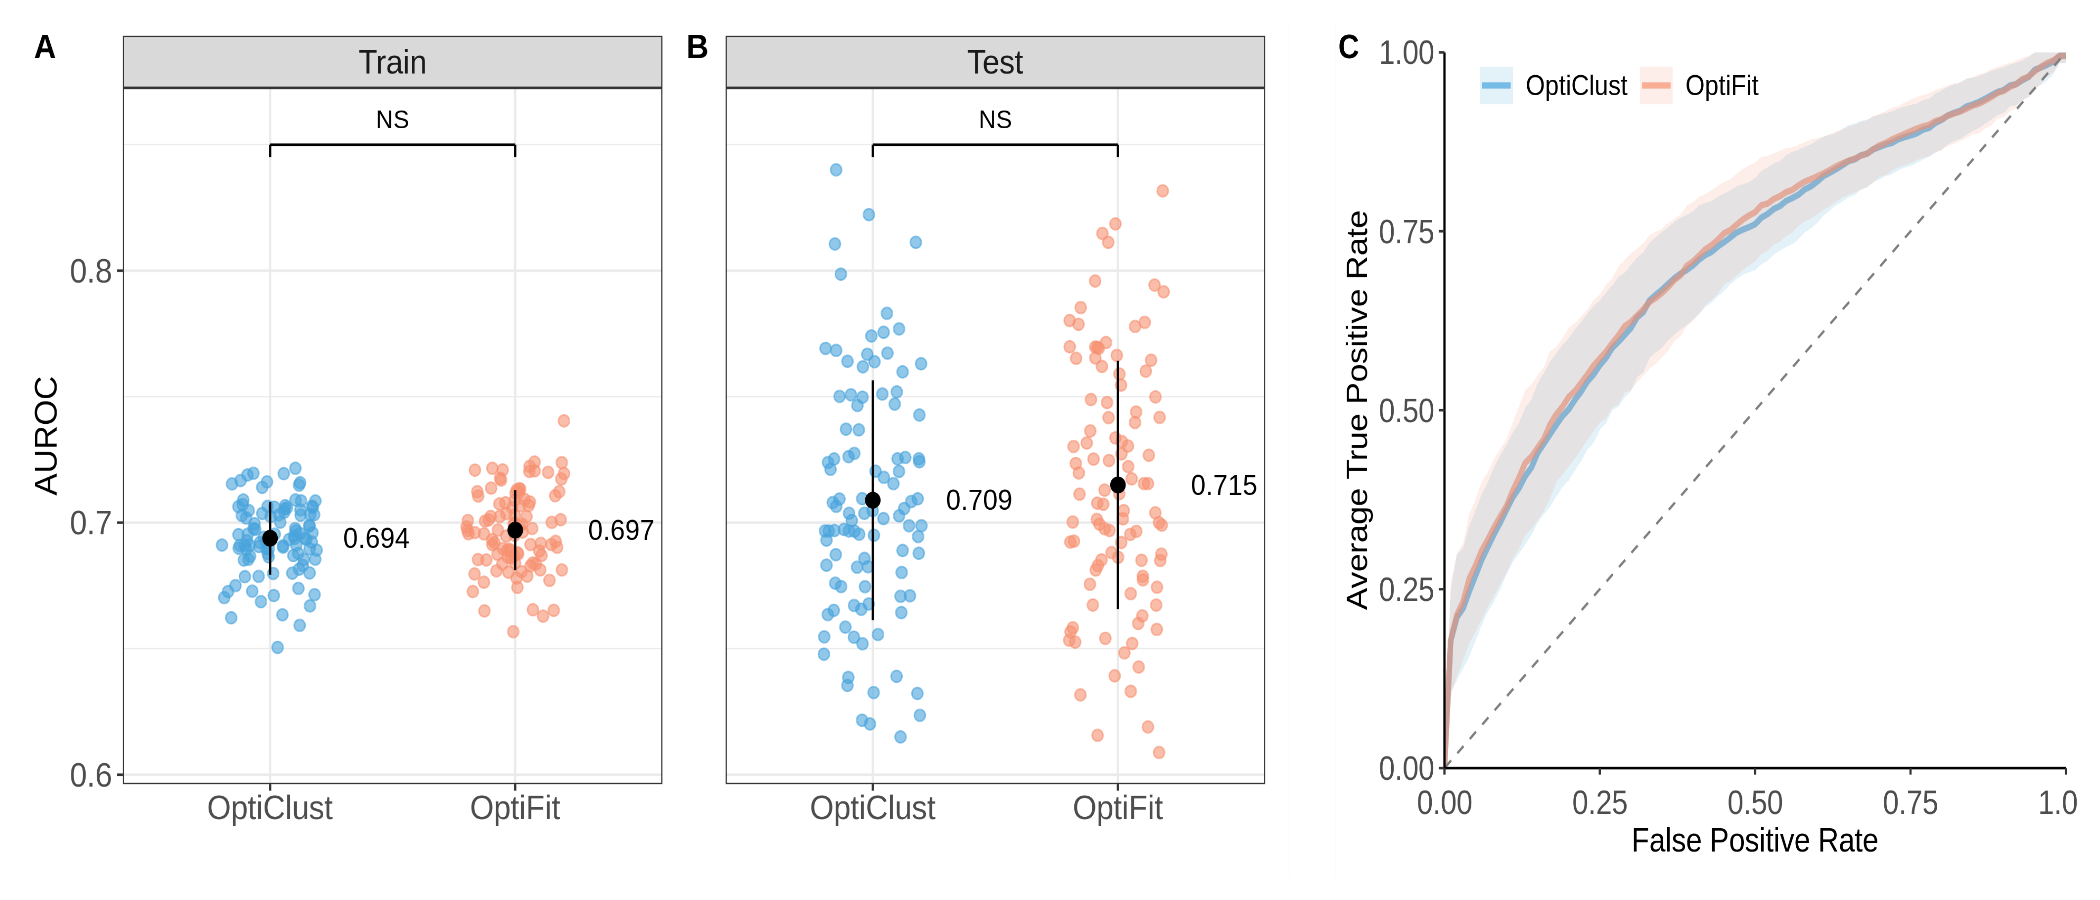
\includegraphics{figures/fig2.png}

\textbf{Figure 2: Model perfomance of OptiFit self-reference workflow is
as good or better than other methods.} \textbf{A)} Area under the
receiver operating characteristic (AUROC) curve during cross-validation
(train) for the various workflows. \textbf{B)} AUROC on the test data
for the various workflows. The mean and standard deviation of the AUROC
is represented by the black dot and whiskers in panels A and B. The mean
AUROC is printed below the points. \textbf{C)} Averaged receiver
operating characteristic (ROC) curves. Lines represent the average true
positive rate for the range of false positive rates.

\end{document}
